\chapter{PCB 2.0 设计和测试}
\label{cha:PCB-v2}

本章设计源文件和历史版本详见\url{https://github.com/TingliangZhang/Misaka-PCB-v2}

\section{需要解决的问题}

在测试版本的PCB(PCB v1)中出现了不少经过测试发现的问题,在第二版本中尽可能予以纠正:

\begin{itemize}
    \item ATmega2560的晶振封装无法手焊,而且不在嘉立创基础库里,不方便SMT
    \item PowerSTEP01过于昂贵,而且极难手动贴片。
\end{itemize}

\section{设计环境的更改}

PCB的设计依赖电子设计自动化(英语:Electronic design automation,缩写:EDA)软件。

当初绘制PCB v1时使用的时Altium Designer 20.0.9集成开发环境。

由于AD20是商业付费EDA软件,而且之前的绘制使用了Altium Live 在线供应商封装库,可移植性和便携性不是很好,即使生成了Integrated Library,也很难找到成套的规范化封装。另外AD20的源文件不是普通编辑器可以打开的文本,这使得Git代码管理变得困难。

基于以上考量,改用KiCAD开源EDA软件进行目前及将来的电路设计,如图~\ref{fig:kicad_flowchart}。

\begin{figure}[htbp]
    \centering
    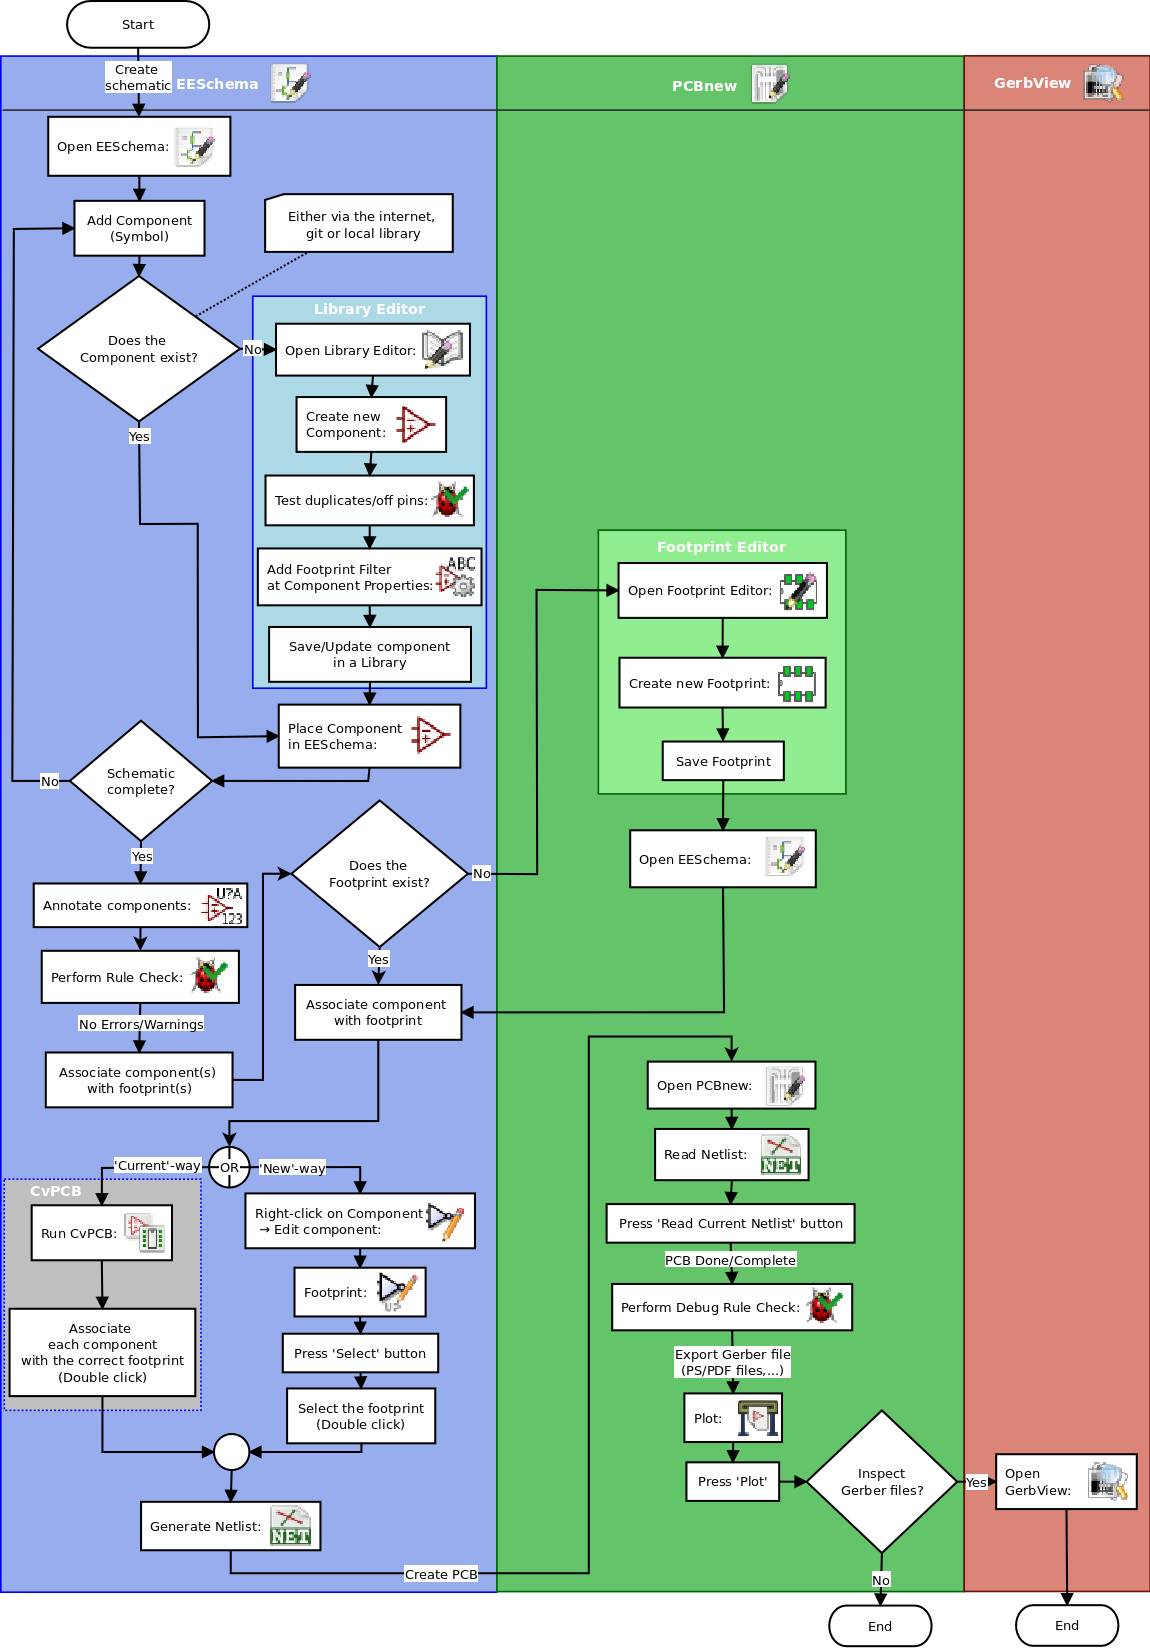
\includegraphics[width=\columnwidth]{kicad_flowchart.png}
    \caption{KiCad Workflow}
    \label{fig:kicad_flowchart}
\end{figure}

\section{定义板子外形轮廓}

在KiCAD PCBNEW编辑器中可以直接在 'Edge.Cuts' 层使用 'Add graphic line or polygon' 定义板子外形轮廓,空格键定义相对坐标原点。

但是只能画简单的直线和圆,而且很麻烦,所以我们使用Fusion 360 导出 DXF 文件定义外形。

如图~\ref{fig:PCB-Measure-v1}。

\begin{figure}[htbp]
    \centering
    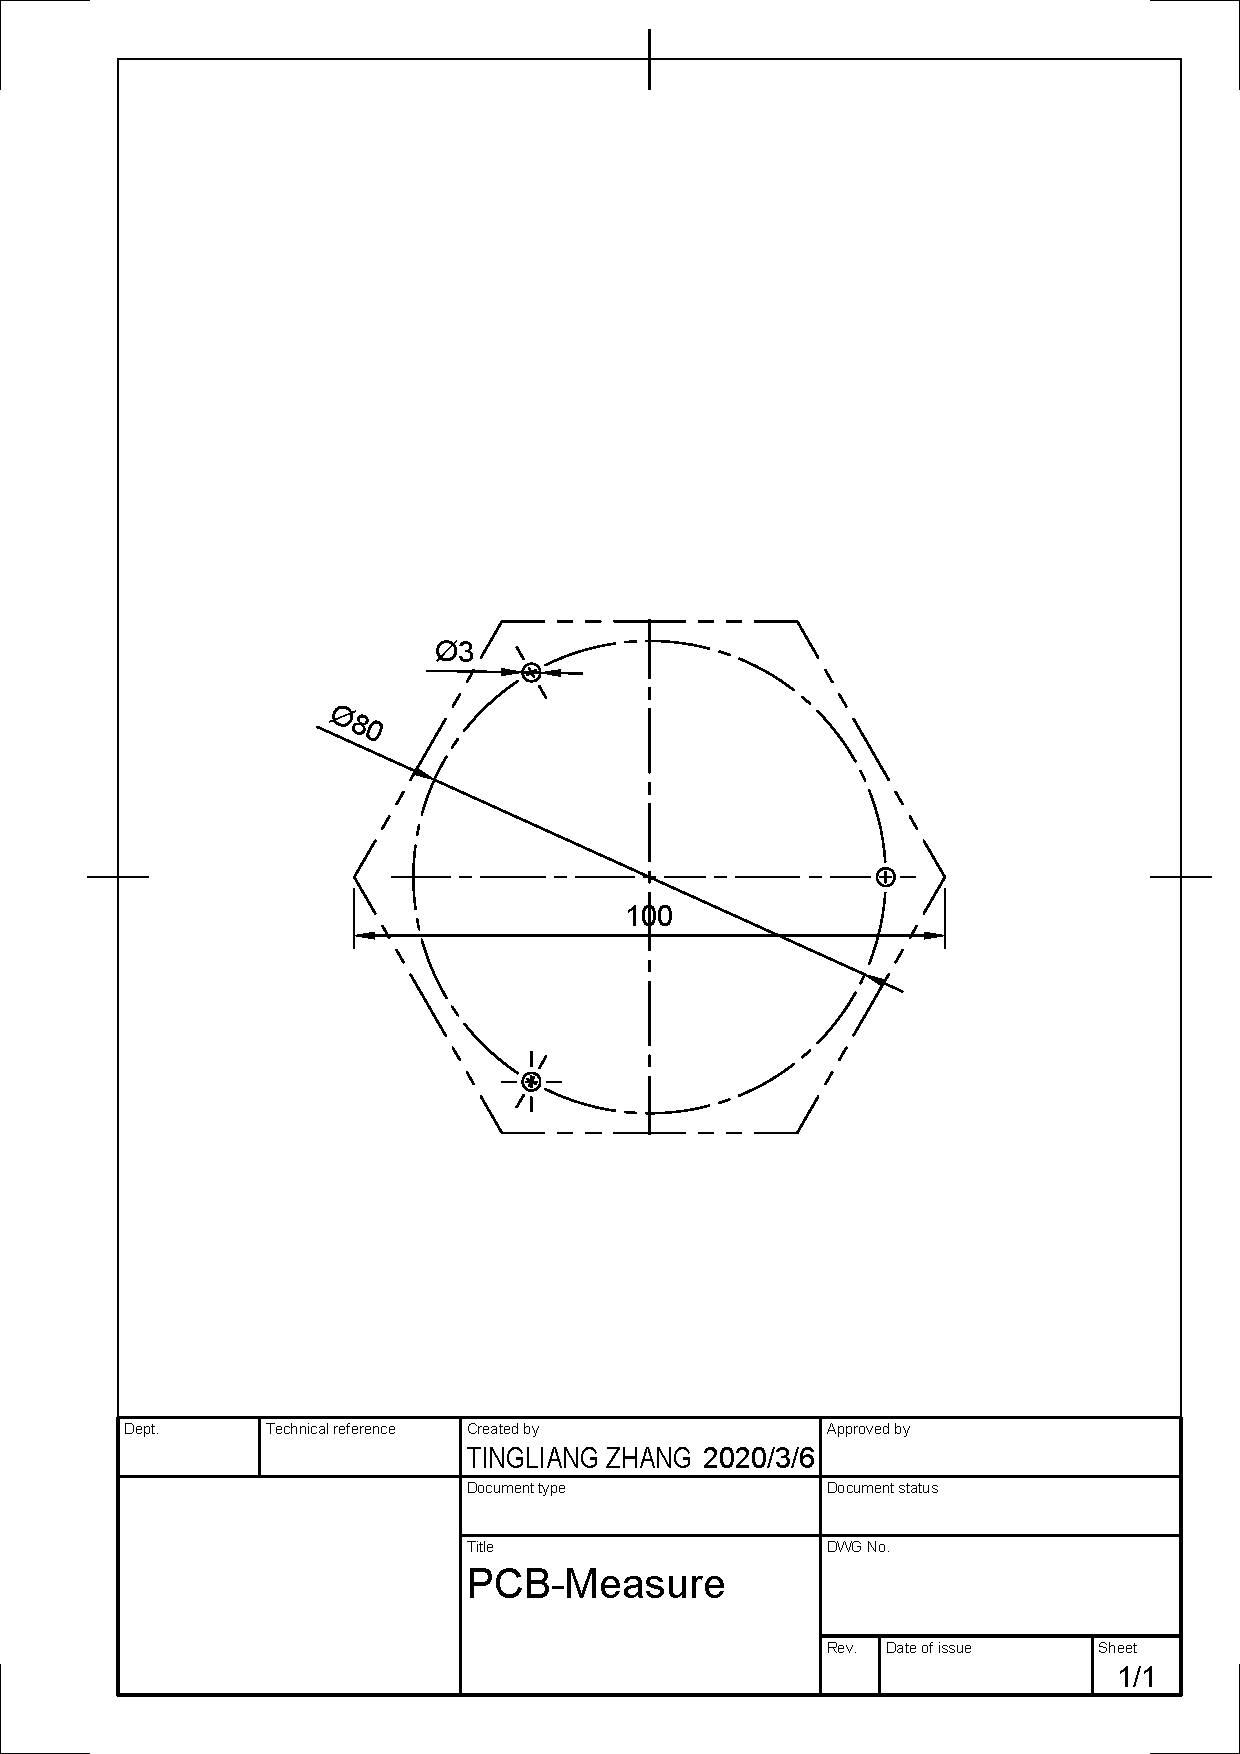
\includegraphics[width=\columnwidth]{PCB-Measure-v1.pdf}
    \caption{PCB DXF}
    \label{fig:PCB-Measure-v1}
\end{figure}



\section{MCU}

参考了Mega Pro Embed CH340G / ATmega2560 board \footnote{\url{https://robotdyn.com/mega-2560-pro-embed-ch340g-atmega2560-16au.html}}的设计,如图~\ref{fig:MEGA-PRO-CH340GATmega2560}。

\begin{figure}[htbp]
    \centering
    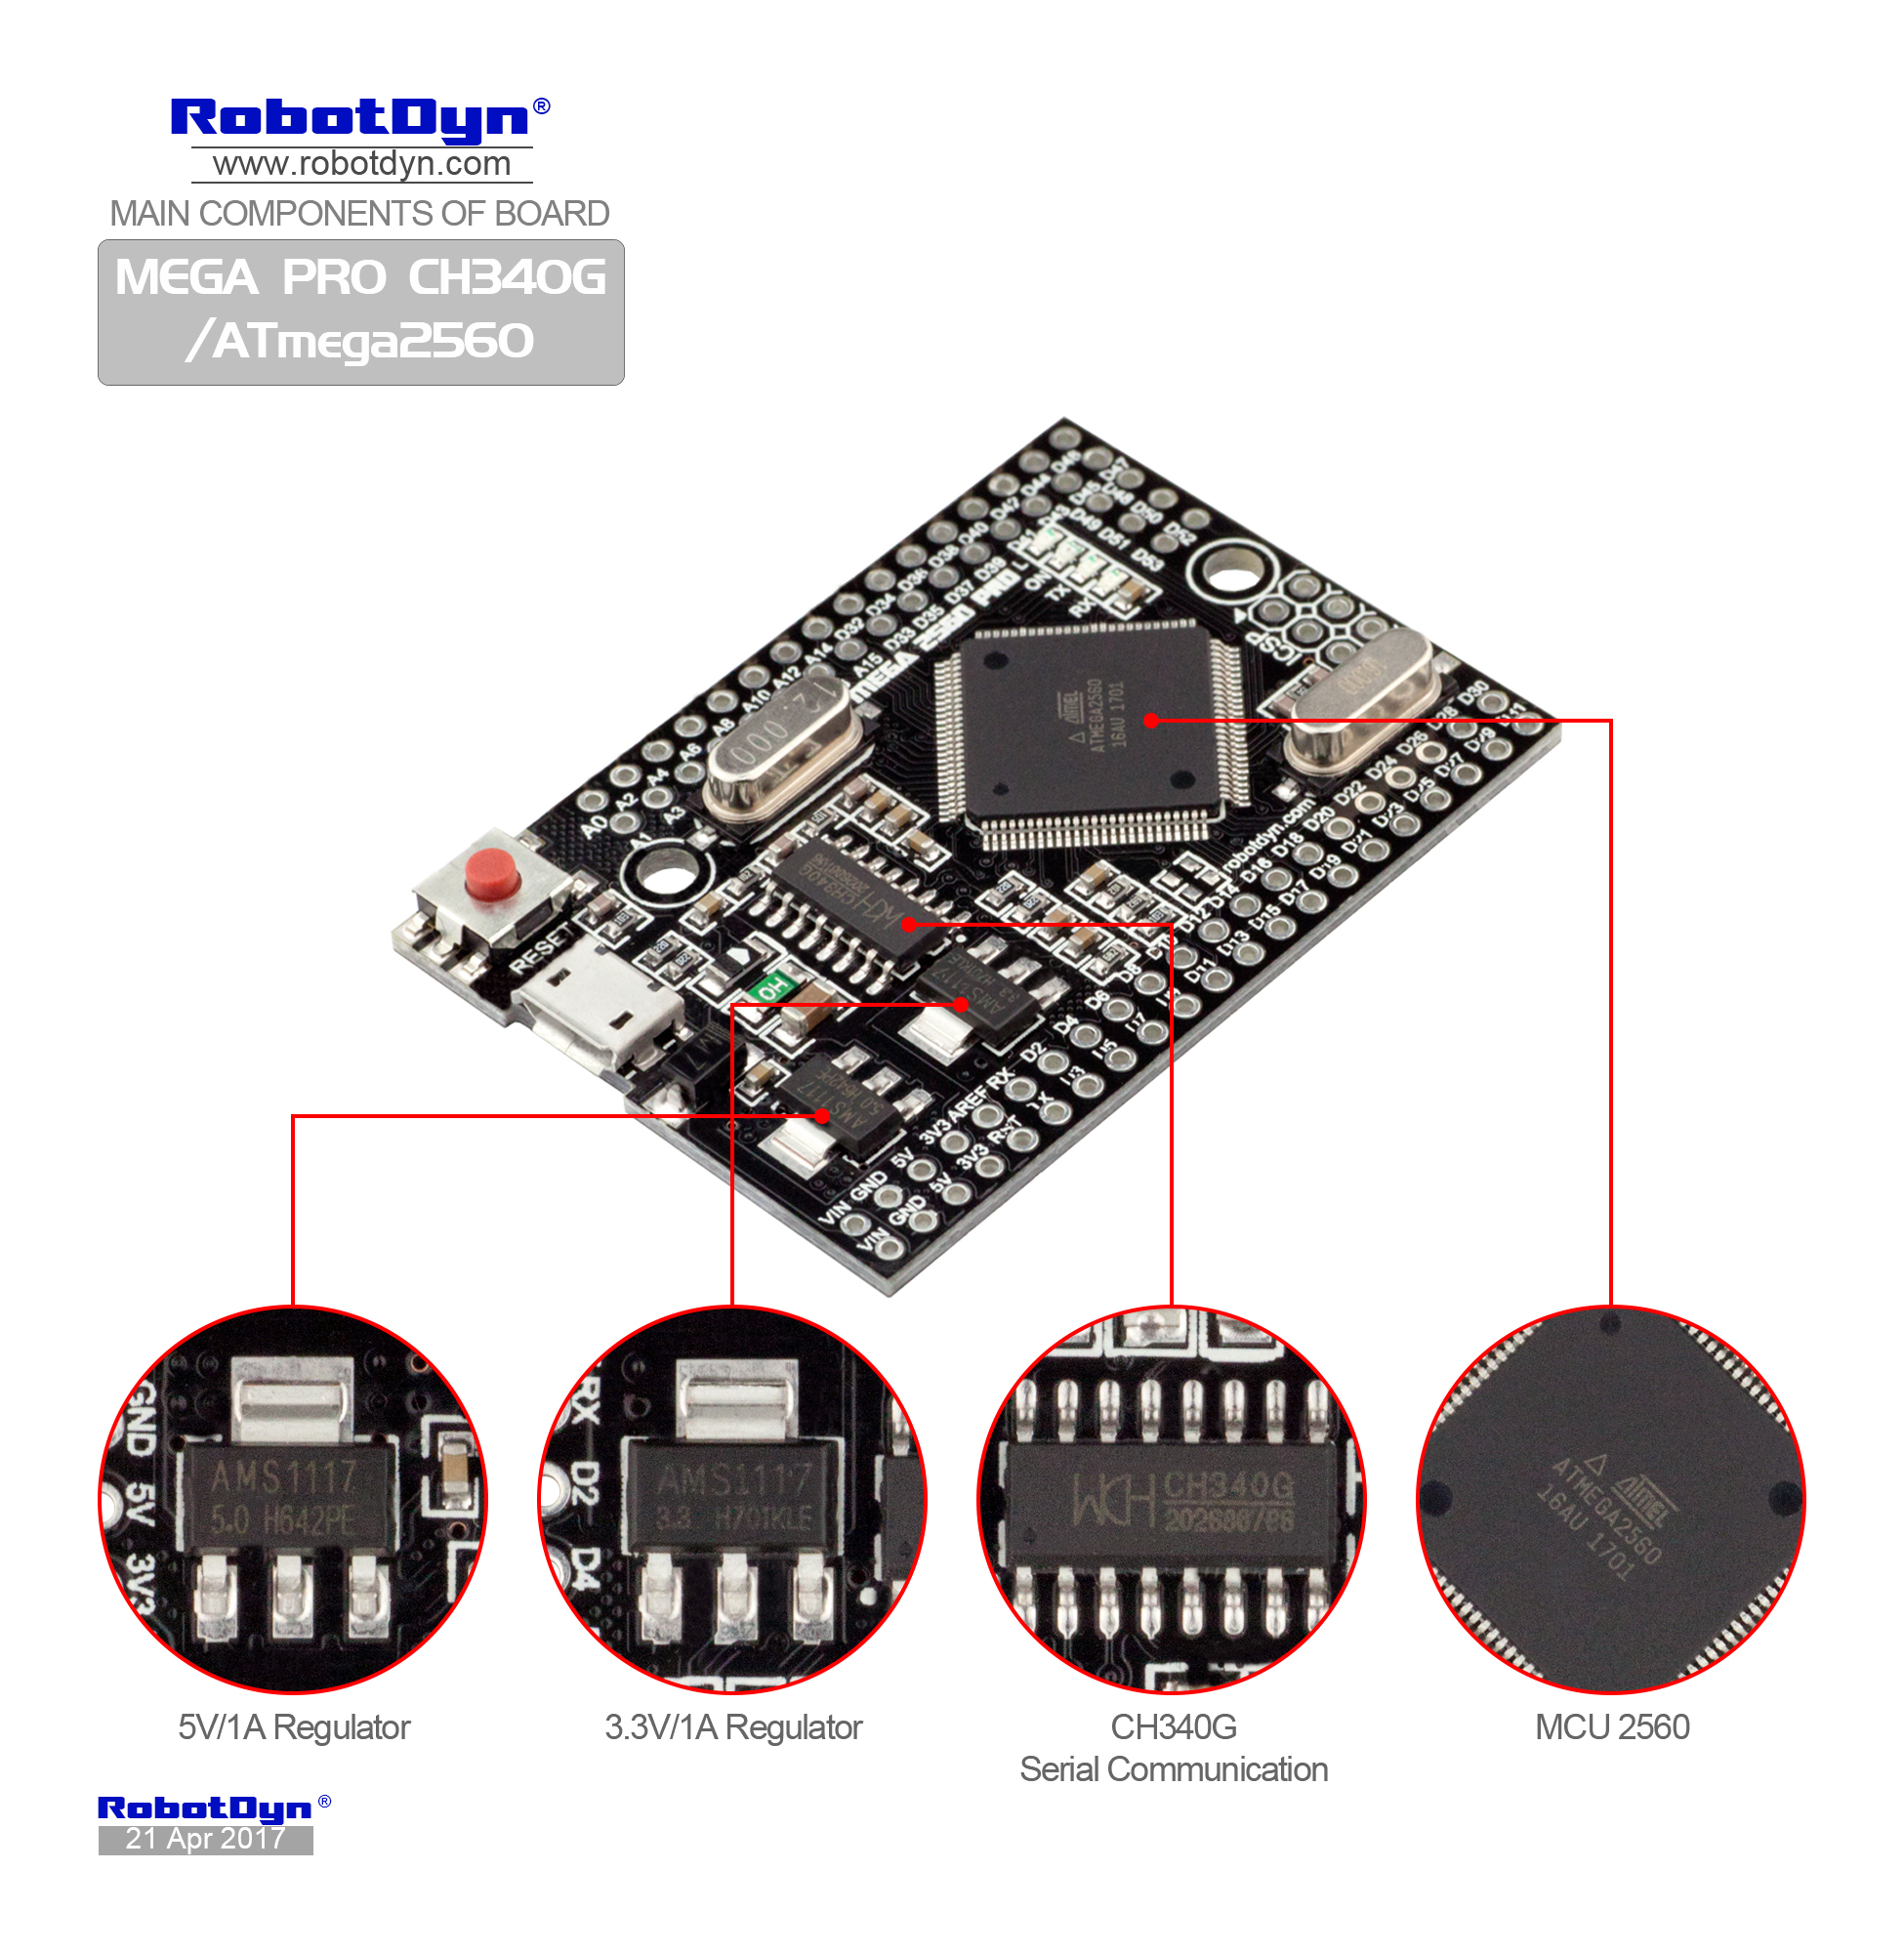
\includegraphics[width=\columnwidth]{MEGA-PRO-CH340GATmega2560.jpg}
    \caption{Mega Pro Embed CH340G / ATmega2560}
    \label{fig:MEGA-PRO-CH340GATmega2560}
\end{figure}


\section{晶振}

由于陶瓷谐振器大多需要外加电容,且封装很难拿手焊,所以选用陶瓷振荡子。

MURATA的 CSTLS16M0X51-A0 \footnote{\url{https://www.murata.com/zh-cn/products/productdetail?partno=CSTLS16M0X51-B0}}。

村田的CSTLS系列陶瓷振荡子(CERALOCK)特征如下:

\begin{enumerate}
    \item 无需外部负载电容器即可构建振荡电路。系列产品拥有内置电容值各不相同的各种型号,可适用于各种集成电路。
    \item 在宽温度范围内稳定。
    \item 结构小巧、重量轻并表现出优异的耐冲击性能。
    \item 可以设计用无需调校的振荡器电路
    \item 性价比高,可用性可靠。
\end{enumerate}



\section{USB UART 异步串行数据传输芯片}

USB转UART芯片稳定程度和价格均为FT232>CH340>PL2303。

FT232RL-REEL价格最贵,1片要27.61,1000+批量价格也要16.24每个。FT232RL/BL的优势就FTDI一直在更新驱动发布在官网,驱动经过微软认证,兼容性最好。内部固化了USB底层协议,转出来的是虚拟串口,可以固定COM口号。电路简单,数据传输稳定性好。FT232RL自带晶振,可以转RS232/TTL(常用)及RS422,RS485 高端市场专用。

PL2303最便宜,但波特率在115200时就有可能出现延迟。

经过测试,CH340\footnote{\url{http://www.wch.cn/products/CH340.html}}可以满足需求,且批量购买1000+只要1.47一片。

CH340C内置晶振,最为合适。

下图是统一供电方式下MCU 单片机通过TTL 串口连接CH340 芯片实现USB通讯的参考电路。该产品选择自供电方式,VCC 支持5V 或者3.3V(VCC 为3.3V 时V3 需短接到VCC),完全不使用USB 总线电源VBUS(如有需要MCU可以通过I/O 串电阻后检测其是否有效)。CH340 与MCU 使用同一电源VCC,所以CH340与MCU 之间不存在双电源通过I/O相互电流倒灌的情形。

CH340没有使用到的信号线都可以悬空。对于CH340C/N/K/E/B 芯片,无需X6 和C17 及C18。

\section{供电}

考虑使用USB PD

USB PD等多快充协议芯片CH236\footnote{\url{http://www.wch.cn/products/CH236.html}}








\section{布线}

Press W or select Custom Track Width from the context menu to type in a custom track width/via size.

To activate the router tool press the Interactive Router button Interactive Router Button or the X key. 

Pressing V or selecting Place Through Via from the context menu while routing a track attaches a via at the end of the trace being routed. Pressing V again disables via placement. Clicking in any spot establishes the via and continues routing (unless 'Shift' is held).

Pressing / or selecting Switch Track Posture from the context menu toggles the direction of the initial track segment between straight or diagonal.

The router can drag track segments, corners and vias. To drag an item, click on it with Ctrl key pressed, hover the mouse and press G or select Drag Track/Via from the context menu.